% Three-panel numerical GEXIT figure.
% Requires \usepackage{pgfplots} and \pgfplotsset{compat=1.18}.
\begin{figure*}[t]
\centering
\begin{minipage}[t]{0.315\textwidth}
\centering
% Compact PGFPlots panel for the surface5 BSC bit-scale decomposition.
% Requires \usepackage{pgfplots} and \pgfplotsset{compat=1.18}.
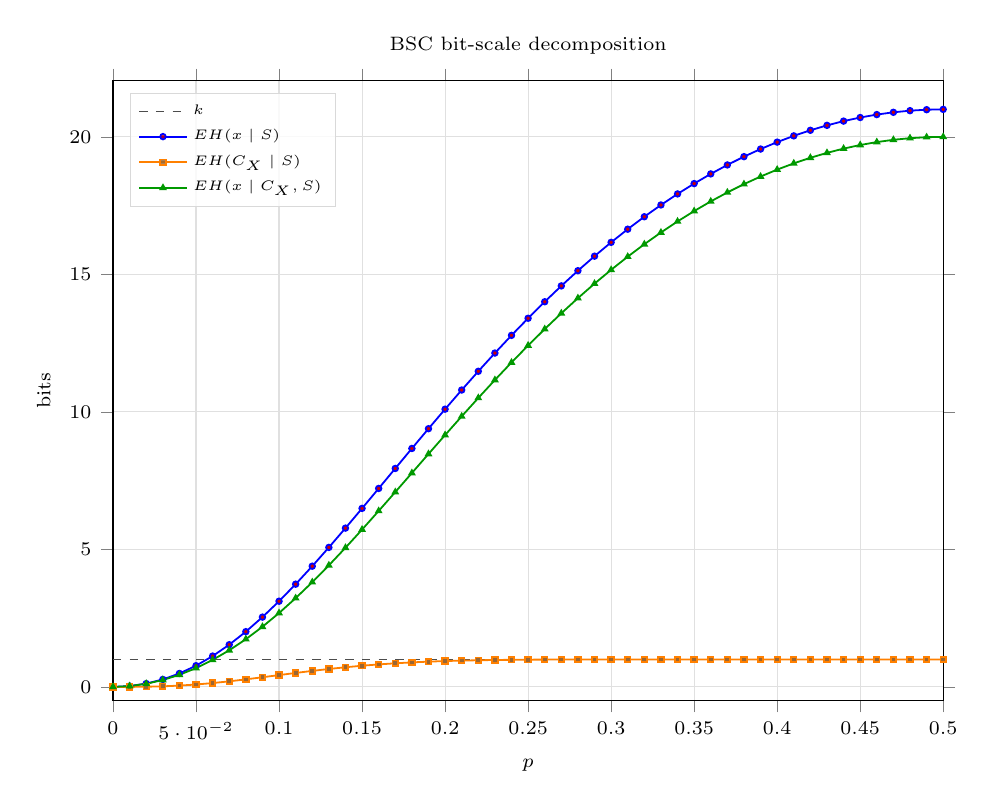
\begin{tikzpicture}
\begin{axis}[
  name=surfaceFiveBSCBitScaleAxis,
  width=\linewidth,
  height=0.78\linewidth,
  title={BSC bit-scale decomposition},
  title style={font=\scriptsize},
  xlabel={$p$},
  ylabel={bits},
  xmin=0, xmax=0.5,
  ymin=-0.5, ymax=22.05,
  grid=both,
  major grid style={black!12},
  minor grid style={black!6},
  tick align=outside,
  tick label style={font=\scriptsize},
  label style={font=\scriptsize},
  legend cell align={left},
  legend style={draw=black!15, fill=white, fill opacity=0.82, text opacity=1, at={(0.02,0.98)}, anchor=north west, font=\tiny},
]
\addplot[black!70, dashed, line width=0.55pt] coordinates {(0,1) (0.5,1)};
\addlegendentry{$k$}
\addplot+[color=blue, mark=*, mark size=1.0pt, line width=0.65pt]
coordinates {(0,0) (0.01,0.0309769830461) (0.02,0.120831945811) (0.03,0.272361948826) (0.04,0.488797485428) (0.05,0.771876603271) (0.06,1.12138210074) (0.07,1.53513383979) (0.08,2.00921740614) (0.09,2.53833335165) (0.1,3.11619011785) (0.11,3.73588882484) (0.12,4.39026752796) (0.13,5.07218771739) (0.14,5.77475710997) (0.15,6.49149052908) (0.16,7.21641542739) (0.17,7.94413101518) (0.18,8.66983065584) (0.19,9.38929675608) (0.2,10.0988762848) (0.21,10.7954436608) (0.22,11.4763563061) (0.23,12.1394068298) (0.24,12.7827746676) (0.25,13.4049790888) (0.26,14.0048347886) (0.27,14.5814107721) (0.28,15.1339928838) (0.29,15.6620500896) (0.3,16.1652044549) (0.31,16.6432046576) (0.32,17.0959028062) (0.33,17.5232342982) (0.34,17.9252004376) (0.35,18.3018535266) (0.36,18.6532841579) (0.37,18.9796104469) (0.38,19.2809689634) (0.39,19.5575071428) (0.4,19.8093769779) (0.41,20.0367298149) (0.42,20.2397120932) (0.43,20.4184618923) (0.44,20.5731061599) (0.45,20.7037585141) (0.46,20.8105175262) (0.47,20.8934654027) (0.48,20.9526669995) (0.49,20.9881691122) (0.5,21)};
\addlegendentry{$\mathbb{E}H(x\mid S)$}
\addplot+[color=orange, mark=square*, mark size=1.0pt, line width=0.65pt]
coordinates {(0,0) (0.01,0.000853674247968) (0.02,0.00660709261872) (0.03,0.0214113132062) (0.04,0.048071359864) (0.05,0.0877491333268) (0.06,0.14002193905) (0.07,0.203174747096) (0.08,0.274607361009) (0.09,0.351261836865) (0.1,0.43000529969) (0.11,0.507931588993) (0.12,0.582568205144) (0.13,0.651991518033) (0.14,0.714863375384) (0.15,0.770407168315) (0.16,0.818342437036) (0.17,0.858795564465) (0.18,0.89220114361) (0.19,0.919205080745) (0.2,0.94057700689) (0.21,0.957136478236) (0.22,0.969694931964) (0.23,0.979013476262) (0.24,0.985775294932) (0.25,0.990570652886) (0.26,0.993892094798) (0.27,0.996137332654) (0.28,0.997617430782) (0.29,0.998568150495) (0.3,0.999162660096) (0.31,0.999524210878) (0.32,0.999737791171) (0.33,0.999860164439) (0.34,0.999928040662) (0.35,0.999964397021) (0.36,0.999983141502) (0.37,0.999992404846) (0.38,0.999996768766) (0.39,0.99999871448) (0.4,0.999999527815) (0.41,0.999999842584) (0.42,0.999999953468) (0.43,0.9999999882) (0.44,0.999999997554) (0.45,0.999999999616) (0.46,0.99999999996) (0.47,0.999999999998) (0.48,1) (0.49,1) (0.5,1)};
\addlegendentry{$\mathbb{E}H(C_X\mid S)$}
\addplot+[color=green!60!black, mark=triangle*, mark size=1.0pt, line width=0.65pt]
coordinates {(0,0) (0.01,0.0301233087981) (0.02,0.114224853192) (0.03,0.25095063562) (0.04,0.440726125564) (0.05,0.684127469945) (0.06,0.981360161694) (0.07,1.33195909269) (0.08,1.73461004513) (0.09,2.18707151478) (0.1,2.68618481816) (0.11,3.22795723585) (0.12,3.80769932281) (0.13,4.42019619936) (0.14,5.05989373459) (0.15,5.72108336076) (0.16,6.39807299035) (0.17,7.08533545071) (0.18,7.77762951223) (0.19,8.47009167534) (0.2,9.15829927793) (0.21,9.83830718256) (0.22,10.5066613741) (0.23,11.1603933536) (0.24,11.7969993726) (0.25,12.4144084359) (0.26,13.0109426938) (0.27,13.5852734395) (0.28,14.1363754531) (0.29,14.6634819391) (0.3,15.1660417948) (0.31,15.6436804468) (0.32,16.096165015) (0.33,16.5233741337) (0.34,16.9252723969) (0.35,17.3018891296) (0.36,17.6533010164) (0.37,17.9796180421) (0.38,18.2809721946) (0.39,18.5575084283) (0.4,18.8093774501) (0.41,19.0367299723) (0.42,19.2397121397) (0.43,19.4184619041) (0.44,19.5731061624) (0.45,19.7037585145) (0.46,19.8105175262) (0.47,19.8934654027) (0.48,19.9526669995) (0.49,19.9881691122) (0.5,20)};
\addlegendentry{$\mathbb{E}H(x\mid C_X,S)$}
\end{axis}
\end{tikzpicture}

{\footnotesize (a) BSC bit-scale decomposition}
\end{minipage}\hfill
\begin{minipage}[t]{0.315\textwidth}
\centering
% Compact PGFPlots panel for Surface BSC GEXIT derivatives.
% Requires \usepackage{pgfplots} and \pgfplotsset{compat=1.18}.
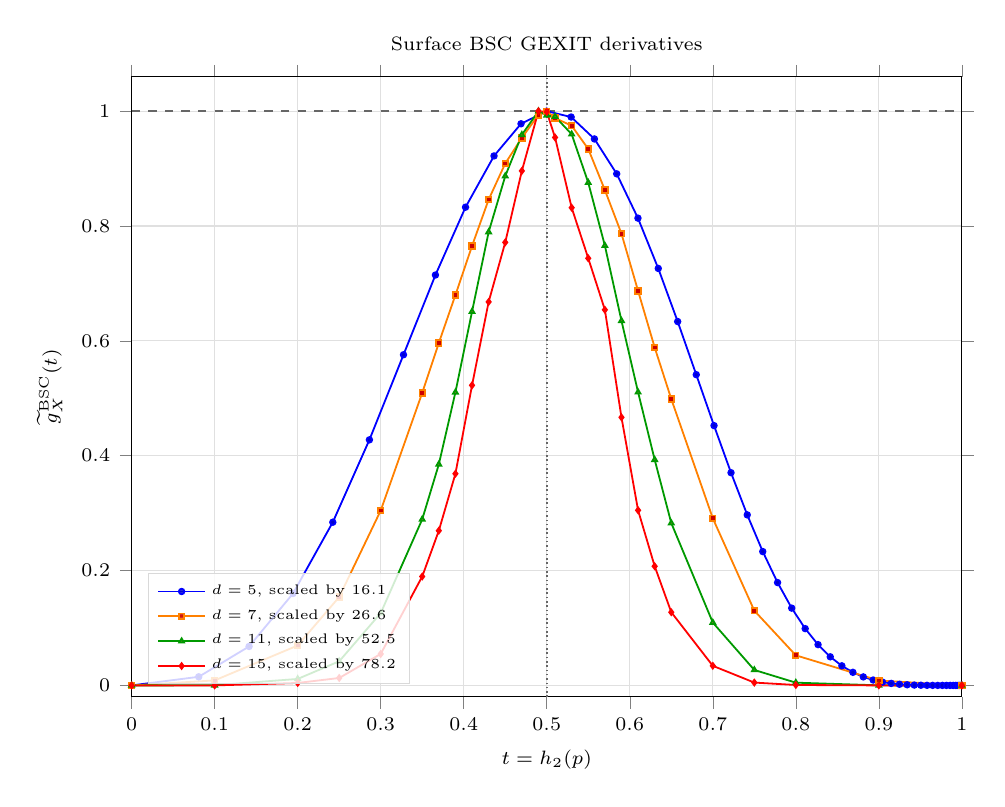
\begin{tikzpicture}
\begin{axis}[
  name=scaledBSCGEXITSurfaceCodesCompact,
  width=\linewidth,
  height=0.78\linewidth,
  title={Surface BSC GEXIT derivatives},
  title style={font=\scriptsize},
  xlabel={$t=h_2(p)$},
  ylabel={$\widetilde g_X^{\rm BSC}(t)$},
  xmin=0, xmax=1,
  ymin=-0.02, ymax=1.06,
  grid=both,
  major grid style={black!12},
  minor grid style={black!6},
  tick align=outside,
  tick label style={font=\scriptsize},
  label style={font=\scriptsize},
  legend cell align={left},
  legend style={draw=black!15, fill=white, fill opacity=0.82, text opacity=1, at={(0.02,0.02)}, anchor=south west, font=\tiny},
]
\addplot[black!60, densely dotted, line width=0.55pt, forget plot] coordinates {(0.5,-0.02) (0.5,1.06)};
\addplot[black!60, dashed, line width=0.55pt, forget plot] coordinates {(0,1) (1,1)};
\addplot+[color=blue, mark=*, mark size=1.0pt, line width=0.65pt]
coordinates {(0,0) (0.0807931358959,0.0150084965486) (0.141440542542,0.0678598992895) (0.194391857832,0.160062893284) (0.242292189082,0.284209247039) (0.286396957116,0.427666640698) (0.327444919154,0.5758242527) (0.3659236509,0.714713391308) (0.402179190202,0.832817118697) (0.436469817064,0.922058340471) (0.468995593589,0.978080835515) (0.499915958165,1) (0.529360865287,0.989813190223) (0.557438185028,0.951640891598) (0.584238811643,0.890934838673) (0.609840304716,0.813749059119) (0.634309554641,0.726131982614) (0.657704778744,0.633666242091) (0.680077045728,0.541159123202) (0.701471459884,0.452470693822) (0.721928094887,0.370457456164) (0.741482739931,0.297005485624) (0.760167502962,0.233126951452) (0.778011303547,0.179096276365) (0.795040279385,0.134605836863) (0.811278124459,0.0989251658741) (0.826746372493,0.0710515251515) (0.841464636208,0.0498431848907) (0.85545081056,0.0341297434636) (0.868721246339,0.022796454474) (0.881290899231,0.0148419400536) (0.893173458378,0.00941089784779) (0.904381457724,0.00580533266894) (0.91492637278,0.00347922103731) (0.924818704973,0.00202211847114) (0.934068055375,0.00113697423916) (0.942683189255,0.000616480143625) (0.950672092687,0.000320971247843) (0.958042022226,0.000159571082972) (0.964799548505,7.51896168136e-05) (0.970950594455,3.32489647039e-05) (0.976500468758,1.36146939678e-05) (0.981453895034,5.06805892557e-06) (0.985815037179,1.67078815901e-06) (0.989587521222,4.69337231444e-07) (0.992774453988,1.05785178373e-07) (0.99537843882,1.72936781607e-08) (0.997401588568,1.69648266606e-09) (0.998845535995,6.5236581209e-11) (0.999711441753,2.52307894475e-13) (1,0)};
\addlegendentry{$d=5$, scaled by $16.1$}
\addplot+[color=orange, mark=square*, mark size=1.0pt, line width=0.65pt]
coordinates {(0,0) (0.1,0.00874083655084) (0.2,0.069519277604) (0.25,0.153993526522) (0.3,0.304565088614) (0.35,0.509384416454) (0.37,0.596428412012) (0.39,0.679860299159) (0.41,0.765368255332) (0.43,0.846034146225) (0.45,0.909003387647) (0.47,0.953510921123) (0.49,0.993571542982) (0.5,1) (0.51,0.98793542682) (0.53,0.974706255802) (0.55,0.934207329936) (0.57,0.862709915391) (0.59,0.786624825435) (0.61,0.686982781924) (0.63,0.588496088453) (0.65,0.49870480007) (0.7,0.290975182716) (0.75,0.130217251484) (0.8,0.0523915877492) (0.9,0.00853288554379) (1,0)};
\addlegendentry{$d=7$, scaled by $26.6$}
\addplot+[color=green!60!black, mark=triangle*, mark size=1.0pt, line width=0.65pt]
coordinates {(0,0) (0.1,0.000240029122595) (0.2,0.0112956420106) (0.25,0.0419923234717) (0.3,0.125935317269) (0.35,0.289218789465) (0.37,0.385015910852) (0.39,0.510496580862) (0.41,0.650976893802) (0.43,0.789519824773) (0.45,0.886931364839) (0.47,0.958863827342) (0.49,1) (0.5,0.992767526717) (0.51,0.990505654574) (0.53,0.959935291674) (0.55,0.875561528763) (0.57,0.765884750492) (0.59,0.635052359911) (0.61,0.510607103869) (0.63,0.393044731252) (0.65,0.282690709626) (0.7,0.109483261407) (0.75,0.0269199643642) (0.8,0.0047988769401) (0.9,0.000150122150357) (1,0)};
\addlegendentry{$d=11$, scaled by $52.5$}
\addplot+[color=red, mark=diamond*, mark size=1.0pt, line width=0.65pt]
coordinates {(0,0) (0.1,2.28805935135e-06) (0.2,0.0042734557494) (0.25,0.0129379312566) (0.3,0.0547968058046) (0.35,0.189701989023) (0.37,0.269444943031) (0.39,0.36866935164) (0.41,0.52265135777) (0.43,0.667844411855) (0.45,0.771531402938) (0.47,0.895998397032) (0.49,1) (0.5,0.998747660336) (0.51,0.95421135537) (0.53,0.831943730372) (0.55,0.743813671081) (0.57,0.654166521537) (0.59,0.466818015439) (0.61,0.304973946397) (0.63,0.207498635762) (0.65,0.127420162371) (0.7,0.0341223878532) (0.75,0.00495582692843) (0.8,0.000738543126851) (0.9,9.82119444954e-06) (1,0)};
\addlegendentry{$d=15$, scaled by $78.2$}
\end{axis}
\end{tikzpicture}

{\footnotesize (b) BSC GEXIT derivatives}
\end{minipage}\hfill
\begin{minipage}[t]{0.315\textwidth}
\centering
% Compact PGFPlots panel for Surface depolarizing GEXIT derivatives.
% Requires \usepackage{pgfplots} and \pgfplotsset{compat=1.18}.
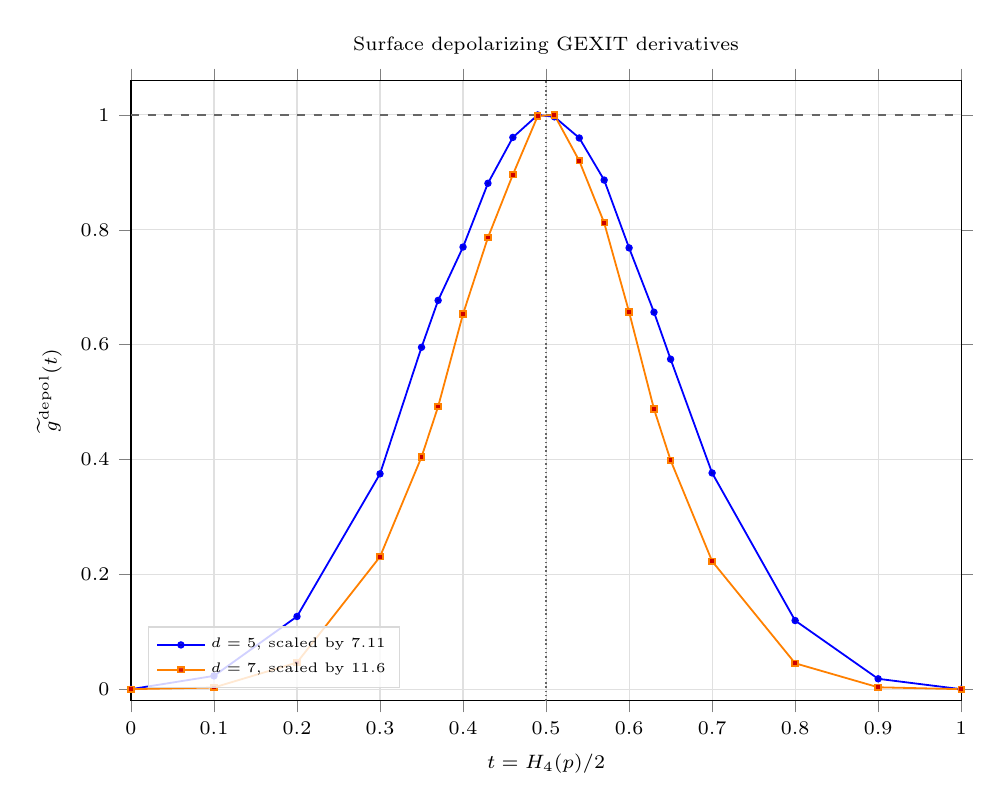
\begin{tikzpicture}
\begin{axis}[
  name=scaledDepolarizingGEXITSurfaceCodesCompact,
  width=\linewidth,
  height=0.78\linewidth,
  title={Surface depolarizing GEXIT derivatives},
  title style={font=\scriptsize},
  xlabel={$t=H_4(p)/2$},
  ylabel={$\widetilde g^{\rm depol}(t)$},
  xmin=0, xmax=1,
  ymin=-0.02, ymax=1.06,
  grid=both,
  major grid style={black!12},
  minor grid style={black!6},
  tick align=outside,
  tick label style={font=\scriptsize},
  label style={font=\scriptsize},
  legend cell align={left},
  legend style={draw=black!15, fill=white, fill opacity=0.82, text opacity=1, at={(0.02,0.02)}, anchor=south west, font=\tiny},
]
\addplot[black!60, densely dotted, line width=0.55pt, forget plot] coordinates {(0.5,-0.02) (0.5,1.06)};
\addplot[black!60, dashed, line width=0.55pt, forget plot] coordinates {(0,1) (1,1)};
\addplot+[color=blue, mark=*, mark size=1.0pt, line width=0.65pt]
coordinates {(0,0) (0.1,0.0231252013791) (0.2,0.126603002342) (0.3,0.375012534461) (0.35,0.595409728769) (0.37,0.677070325975) (0.4,0.769998155027) (0.43,0.881000538857) (0.46,0.960872147817) (0.49,1) (0.51,0.996728698583) (0.54,0.959878469441) (0.57,0.886582284073) (0.6,0.76850463298) (0.63,0.656474564855) (0.65,0.574721364111) (0.7,0.376565494666) (0.8,0.119534693579) (0.9,0.0180571703987) (1,0)};
\addlegendentry{$d=5$, scaled by $7.11$}
\addplot+[color=orange, mark=square*, mark size=1.0pt, line width=0.65pt]
coordinates {(0,0) (0.1,0.00295645955089) (0.2,0.0463368250444) (0.3,0.230674423002) (0.35,0.404356116017) (0.37,0.492124430801) (0.4,0.653376106363) (0.43,0.786462010477) (0.46,0.896005711653) (0.49,0.998262837311) (0.51,1) (0.54,0.920114970537) (0.57,0.812139542886) (0.6,0.656859913063) (0.63,0.487919909896) (0.65,0.398650257397) (0.7,0.22283287194) (0.8,0.0451166562625) (0.9,0.00332813163872) (1,0)};
\addlegendentry{$d=7$, scaled by $11.6$}
\end{axis}
\end{tikzpicture}

{\footnotesize (c) Depolarizing GEXIT derivatives}
\end{minipage}
\caption{Surface-code GEXIT numerics.  Panel (a) shows the BSC bit-scale
decomposition for the $d=5$ surface code.  Panel (b) overlays scaled BSC
component GEXIT derivatives against $t=h_2(p)$.  Panel (c) overlays scaled
depolarizing GEXIT derivatives against normalized Pauli entropy
$t=H_4(p)/2$.  Legend scaling is for visual comparison only; unscaled areas
are recorded in the accompanying scaling CSV files.}
\label{fig:surface-gexit-numerics}
\end{figure*}
